\hiddenref{}

\section{Introduction\label{introduction}}

% \IEEEPARstart{A}{mong} 

\subsection{Motivation and Our Work}

The NIST report in submitted for the US Congress \cite{2002SUMMARYON} underlines that about $2\%$ of the user population does not have usable fingerprints. NIST studies have also reported false positive identification rate (FPIR) of ten-finger identification in the range of 1.5 to $3.5\%$ on a gallery size of about one million. Similar conclusions have also been reported in a large-scale proof of concept study undertaken by UIDAI [1]. This study indicated that about $1.9\%$ of the subjects cannot be reliably authenticated by only using their fingerprints. One of the key challenges with large scale deployed fingerprint authentication systems is also related to the acquisition of fingerprint images and such sensing requires a fair degree of cooperation from the users. Therefore, it is not uncommon in the literature to report failure to enroll (FTE) rate in the range of $1\%$ to $5\%$ for the fingerprints. 

By incorporating finger knuckle information for user identification, the drawback of currently popular fingerprint only user identification can be complemented. Besides, there are several advantages of the new system. First, data collection facility is easy to set with low cost. Second, data collection procedure is simple. Since the finger knuckle and fingerprint data can be collected simultaneously, no extra time is needed. Third, user will have almost the same user experience without having any confusion. The key idea of this paper is to develop a finger-knuckle assisted fingerprint identification system to significantly improve user identification accuracy without causing additional user inconvenience. In order to achieve this goal, firstly, the fingerprint and finger-knuckle data of each user must be acquired simultaneously and with a single imaging shot; secondly, both fingerprint and finger-knuckle must be accurately segmented and aligned; finally, a dynamic fusion strategy must be introduced to accommodate degradation in the fingerprint and finger-knuckle quality and significantly enhance user the identification capabilities. 

\begin{figure}[!ht]
    \centering
    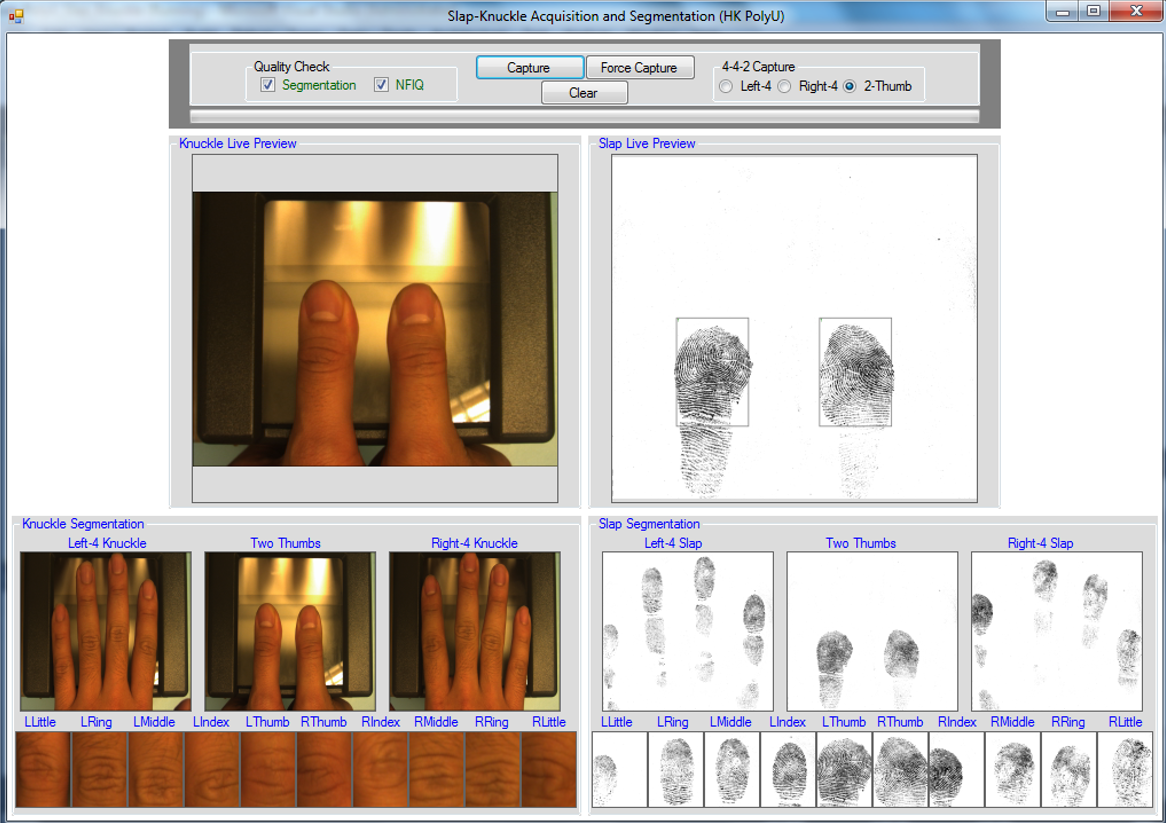
\includegraphics[width=3.4in]{Figures/system.png}
    \caption{Online user authentication using slap-fingerprint and finger-knuckle images: joint user interface developed for the 4-4-2 protocols }
    \label{system}
\end{figure}

The key contributions from this paper can be summarized as follows: 

\begin{itemize}
    \item This paper introduces a new biometric system, i.e. finger-knuckle assisted fingerprint identification system, to address current limitations from widely deployed slap-fingerint sensors at border crossings and for national ID progarms. This system simultaneously acquires fingerprint and finger-knuckle images with a single imaging shot, with no additional user inconvenience or degradation in traffic flow, and can serve as an add-on system for the existing or the deployed slap fingerprint systems. Our research introduces more effective finger knuckle segmentation capabilities, from the finger dorsal images acquired under complex backgrounds, ambient illumination and in presence of multiple finger knuckles that are inherently observed in such simultaneously acquired images. We incorporate dynamic fusion capabilities to address the limitations resulting from the degraded fingerprint or finger-kuckle images. Our experimental results presented in this paper validate the effectiveness of the proposed biometric system for its usage in a range of real-world applications. 
    \item We develop first joint finger-knuckle and fingerprint database which has been acquired from 120 different subjects, using 4-4-2 imaging protocols, and introduce in the public domain. In the best of our knowledge, there no such joint database developed or available so far, and its availability in public domain will help to advance further research and development efforts for the real-applications. 
\end{itemize}


The rest of this paper is organized as follows. Section 2 introduces single-shot imaging based framework for the finger-knuckle assisted slap fingerprint identification. This section also details finger knuckle segmentation strategy developed to automatically segment finger knuckle images from the slap finger dorsal images acquired under complex and ambient imaging backgrounds. Section 3 introduces dynamic scheme to consolidate finger knuckle and fingerprint match scores while Section 4 presents the experimental results. Section 5 presents discussion and the key conclusions of this work are summarized in Section 6.